\documentclass[12pt,a4paper]{report}
\usepackage[utf8]{inputenc}
\usepackage{amsmath}
\usepackage{amsfonts}
\usepackage{amssymb}
\usepackage{amsthm}
\usepackage{hyperref}
\usepackage{mathrsfs}

\usepackage{multicol}
\usepackage{fancyhdr}
\usepackage[inline]{enumitem}
\usepackage{tikz}
\usepackage{tikz-cd}
\usetikzlibrary{calc}
\usetikzlibrary{shapes.geometric}
\usetikzlibrary{positioning}
\usepackage[margin=0.5in]{geometry}
\usepackage{xcolor}

\hypersetup{
    colorlinks=true,
    linkcolor=blue,
    filecolor=magenta,      
    urlcolor=cyan,
    pdftitle={Tensors},
    pdfpagemode=FullScreen,
    }

%\urlstyle{same}

\newcommand{\CLASSNAME}{Math XXXX -- Independent Study: Differential Geometry, Lie Groups}
\newcommand{\STUDENTNAME}{Paul Carmody}
\newcommand{\ASSIGNMENT}{\textit{Basic Category Theory -- Tom Leinster}}
\newcommand{\DUEDATE}{August, 2025}
\newcommand{\PROFESSOR}{Professor Berchenko-Kogan}
\newcommand{\SEMESTER}{Summer 2025}
\newcommand{\SCHEDULE}{TBD}
\newcommand{\ROOM}{Edinburgh}

\newcommand{\MMN}{M_{m\times n}}
\newcommand{\FF}{\mathcal{F}}
\newcommand{\ADJOINT}[2]{\underset{\underset{#2}\longleftarrow}{\overset{\overset{#1}\longrightarrow}\bot }}


\pagestyle{fancy}
\fancyhf{}
\chead{ \fancyplain{}{\CLASSNAME} }
%\chead{ \fancyplain{}{\STUDENTNAME} }
\rhead{\thepage}
\newcommand{\LET}{\text{Let }}
%\newcommand{\IF}{\text{if }}
\newcommand{\AND}{\text{ and }}
\newcommand{\OR}{\text{ or }}
\newcommand{\FORSOME}{\text{ for some }}
\newcommand{\FORALL}{\text{ for all }}
\newcommand{\WHERE}{\text{ where }}
\newcommand{\WTS}{\text{ WTS }}
\newcommand{\WLOG}{\text{ WLOG }}
\newcommand{\BS}{\backslash}
\newcommand{\DEFINE}[1]{\textbf{\emph{#1}}}
\newcommand{\IF}{$(\Rightarrow)$}
\newcommand{\ONLYIF}{$(\Leftarrow)$}
\newcommand{\ITH}{\textsuperscript{th} }
\newcommand{\FST}{\textsuperscript{st} }
\newcommand{\SND}{\textsuperscript{nd} }
\newcommand{\TRD}{\textsuperscript{rd} }
\newcommand{\INV}{\textsuperscript{-1} }

\newcommand{\XXX}{\mathfrak{X}}
\newcommand{\MMM}{\mathfrak{M}}
%\newcommand{\????}{\textfrak{A}}
%\newcommand{\????}{\textgoth{A}}
%\newcommand{\????}{\textswab{A}}

\DeclareMathOperator{\DER}{Der}
\DeclareMathOperator{\SGN}{sgn}

%%%%%%%
% derivatives
%%%%%%%

\newcommand{\PART}[2]{\frac{\partial #1}{\partial #2}}
\newcommand{\SPART}[2]{\frac{\partial^2 #1}{\partial #2^2}}
\newcommand{\DERIV}[2]{\frac{d #1}{d #2}}
\newcommand{\LAPLACIAN}[1]{\frac{\partial^2 #1}{\partial x^2} + \frac{\partial^2 #1}{\partial y^2}}

%%%%%%%
% sum, product, union, intersections
%%%%%%%

\newcommand{\SUM}[2]{\underset{#1}{\overset{#2}{\sum}}}
\newcommand{\PROD}[2]{\underset{#1}{\overset{#2}{\prod}}}
\newcommand{\UNION}[2]{\underset{#1}{\overset{#2}{\bigcup}}}
\newcommand{\INTERSECT}[2]{\underset{#1}{\overset{#2}{\bigcap}}}
\newcommand{\FSUM}{\SUM{n=-\infty}{\infty}}
       

%%%%%%%
% supremum and infimum
%%%%%%%

\newcommand{\SUP}[1]{\underset{#1}\sup \,}
\newcommand{\INF}[1]{\underset{#1}\inf \,}
\newcommand{\MAX}[1]{\underset{#1}\max \,}
\newcommand{\MIN}[1]{\underset{#1}\min \,}

%%%%%%%
% infinite sums, limits
%%%%%%%

\newcommand{\SUMK}{\SUM{k=1}{\infty}}
\newcommand{\SUMN}{\SUM{n=1}{\infty}}
\newcommand{\SUMKZ}{\SUM{k=0}{\infty}}
\newcommand{\LIM}[1]{\underset{#1}\lim\,}
\newcommand{\IWOB}[1]{\LIM{#1 \to \infty}}
\newcommand{\LIMK}{\IWOB{k}}
\newcommand{\LIMN}{\IWOB{n}}
\newcommand{\LIMX}{\IWOB{x}}
\newcommand{\NIWOB}{\LIM{n \to \infty}}
\newcommand{\LIMSUPK}{\underset{k\to\infty}\limsup \,}
\newcommand{\LIMSUPN}{\underset{n\to\infty}\limsup \,}
\newcommand{\LIMINFK}{\underset{k\to\infty}\liminf \,}
\newcommand{\LIMINFN}{\underset{n\to\infty}\liminf \,}
\newcommand{\ROOTRULE}[1]{\LIMSUPK \BARS{#1}^{1/k}}

\newcommand{\CUPK}{\bigcup_{k=1}^{\infty}}
\newcommand{\CAPK}{\bigcap_{k=1}^{\infty}}
\newcommand{\CUPN}{\bigcup_{n=1}^{\infty}}
\newcommand{\CAPN}{\bigcap_{n=1}^{\infty}}

%%%%%%%
% number systems (real, rational, etc.)
%%%%%%%

\newcommand{\REALS}{\mathbb{R}}
\newcommand{\RATIONALS}{\mathbb{Q}}
\newcommand{\IRRATIONALS}{\REALS \backslash \RATIONALS}
\newcommand{\INTEGERS}{\mathbb{Z}}
\newcommand{\NUMBERS}{\mathbb{N}}
\newcommand{\COMPLEX}{\mathbb{C}}
\newcommand{\DISC}{\mathbb{D}}
\newcommand{\HPLANE}{\mathbb{H}}

\newcommand{\R}{\mathbb{R}}
\newcommand{\Q}{\mathbb{Q}}
\newcommand{\Z}{\mathbb{Z}}
\newcommand{\N}{\mathbb{N}}
\newcommand{\C}{\mathbb{C}}
\newcommand{\T}{\mathbb{T}}
\newcommand{\COUNTABLE}{\aleph_0}
\newcommand{\UNCOUNTABLE}{\aleph_1}


%%%%%%%
% Arithmetic/Algebraic operators
%%%%%%%


\DeclareMathOperator{\MOD}{mod}
%\newcommand{\MOD}[1]{\mod #1}
\newcommand{\BAR}[1]{\overline{#1}}
\newcommand{\LCM}{\text{ lcm}}
\newcommand{\ZMOD}[1]{\Z/#1\Z}
\DeclareMathOperator{\VAR}{Var}
%%%%%%%
% complex operators
%%%%%%%

\DeclareMathOperator{\RR}{Re}
%\newcommand{\RE}{\text{Re}}
\DeclareMathOperator{\IM}{Im}
%\newcommand{\IM}{\text{Im}}
\newcommand{\CONJ}[1]{\overline{#1}}
\DeclareMathOperator{\LOG}{Log}
%\newcommand{\LOG}{\text{ Log }}
\newcommand{\RES}[2]{\underset{#1}{\text{res}} #2}

%%%%%%%
% Group operators
%%%%%%%

\newcommand{\AUT}{\text{Aut}\,}
\newcommand{\KER}{\text{ker}\,}
\newcommand{\END}{\text{End}}
\newcommand{\HOM}{\text{Hom}}
\newcommand{\CYCLE}[1]{(\begin{array}{cccccccccc}
		#1
	\end{array})}
\newcommand{\SUBGROUP}{\underset{\text{group}}\subseteq}	
%\newcommand{\SUBGROUP}{\subseteq_g}
\newcommand{\SUBRING}{\underset{\text{ring}}\subseteq}
\newcommand{\SUBMOD}{\underset{\text{mod}}\subseteq}
\newcommand{\SUBFIELD}{\underset{\text{field}}\subseteq}
\newcommand{\ISO}{\underset{\text{iso}}\longrightarrow}
\newcommand{\HOMO}{\underset{\text{homo}}\longrightarrow}

%%%%%%%
% grouping (parenthesis, absolute value, square, multi-level brackets).
%%%%%%%

\newcommand{\PAREN}[1]{\left (\, #1 \,\right )}
\newcommand{\BRACKET}[1]{\left \{\, #1 \,\right \}}
\newcommand{\SQBRACKET}[1]{\left [\, #1 \,\right ]}
\newcommand{\ABRACKET}[1]{\left \langle\, #1 \,\right \rangle}
\newcommand{\BARS}[1]{\left |\, #1 \,\right |}
\newcommand{\DBARS}[1]{\left \| \, #1 \,\right \|}
\newcommand{\LBRACKET}[1]{\left \{ #1 \right .} 
\newcommand{\RBRACKET}[1]{\left . #1 \right \]}
\newcommand{\RBAR}[1]{\left . #1 \, \right |}
\newcommand{\LBAR}[1]{\left | \, #1 \right .}
\newcommand{\BLBRACKET}[2]{\BRACKET{\RBAR{#1}#2}}
\newcommand{\GEN}[1]{\ABRACKET{#1}}
\newcommand{\BINDEF}[2]{\LBRACKET{\begin{array}{ll}
     #1\\
     #2
\end{array}}}

%%%%%%%
% Fourier Analysis
%%%%%%%

\newcommand{\ONEOTWOPI}{\frac{1}{2\pi}}
\newcommand{\FHAT}{\hat{f}(n)}
\newcommand{\FINT}{\int_{-\pi}^\pi}
\newcommand{\FINTWO}{\int_{0}^{2\pi}}
\newcommand{\FSUMN}[1]{\SUM{n=-#1}{#1}}
%\newcommand{\FSUM}{\SUMN{\infty}}
\newcommand{\EIN}[1]{e^{in#1}}
\newcommand{\NEIN}[1]{e^{-in#1}}
\newcommand{\INTALL}{\int_{-\infty}^{\infty}}
\newcommand{\FTINT}[1]{\INTALL #1 e^{2\pi inx\xi} dx}
\newcommand{\GAUSS}{e^{-\pi x^2}}

%%%%%%%
% formatting 
%%%%%%%

\newcommand{\LEFTBOLD}[1]{\noindent\textbf{#1}}
\newcommand{\SEQ}[1]{\{#1\,\}}
\newcommand{\WIP}{\footnote{work in progress}}
\newcommand{\QED}{\hfill\square}
\newcommand{\ts}{\textsuperscript}
\newcommand{\HLINE}{\noindent\rule{7in}{1pt}\\}

%%%%%%%
% Mathematical note taking (definitions, theorems, etc.)
%%%%%%%

\newcommand{\REM}{\noindent\textbf{\\Remark: }}
\newcommand{\DEF}{\noindent\textbf{\\Definition: }}
\newcommand{\THE}{\noindent\textbf{\\Theorem: }}
\newcommand{\COR}{\noindent\textbf{\\Corollary: }}
\newcommand{\LEM}{\noindent\textbf{\\Lemma: }}
\newcommand{\PROP}{\noindent\textbf{\\Proposition: }}
\newcommand{\PROOF}{\noindent\textbf{\\Proof: }}
\newcommand{\EXP}{\noindent\textbf{\\Example: }}
\newcommand{\TRICKS}{\noindent\textbf{\\Tricks: }}


%%%%%%%
% text highlighting
%%%%%%%

\newcommand{\B}[1]{\textbf{#1}}
\newcommand{\CAL}[1]{\mathcal{#1}}
\newcommand{\UL}[1]{\underline{#1}}

%%%%%%
% Linear Algebra
%%%%%%

\newcommand{\COLVECTOR}[1]{\PAREN{\begin{array}{c}
#1
\end{array} }}
\newcommand{\TWOXTWO}[4]{\PAREN{ \begin{array}{c c} #1&#2 \\ #3 & #4 \end{array} }}
\newcommand{\DTWOXTWO}[4]{\BARS{ \begin{array}{c c} #1&#2 \\ #3 & #4 \end{array} }}
\newcommand{\THREEXTHREE}[9]{\PAREN{ \begin{array}{c c c} #1&#2&#3 \\ #4 & #5 & #6 \\ #7 & #8 & #9 \end{array} }}
\newcommand{\DTHREEXTHREE}[9]{\BARS{ \begin{array}{c c c} #1&#2&#3 \\ #4 & #5 & #6 \\ #7 & #8 & #9 \end{array} }}
\newcommand{\NXN}{\PAREN{ \begin{array}{c c c c} 
			a_{11} & a_{12} & \cdots & a_{1n} \\
			a_{21} & a_{22} & \cdots & a_{2n} \\
			\vdots & \vdots & \ddots & a_{1n} \\
			a_{n1} & a_{n2} & \cdots & a_{nn} \\
		\end{array} }}
\newcommand{\SLR}{SL_2(\R)}
\newcommand{\GLR}{GL_2(\R)}
\DeclareMathOperator{\TR}{tr}
\DeclareMathOperator{\BIL}{Bil}
\DeclareMathOperator{\SPAN}{span}

%%%%%%%
%  White space
%%%%%%%

\newcommand{\BOXIT}[1]{\noindent\fbox{\parbox{\textwidth}{#1}}}


\newtheorem{theorem}{Theorem}[section]
\newtheorem{corollary}{Corollary}[theorem]
\newtheorem{lemma}[theorem]{Lemma}

\theoremstyle{definition}
\newtheorem{definition}[theorem]{Definition}
\newtheorem{prop}[theorem]{Proposition}

\theoremstyle{remark}
\newtheorem{remark}[theorem]{Remark}
\newtheorem{example}[theorem]{Example}
%\newtheorem*{proof}[theorem]{Proof}



\newcommand{\RED}[1]{\textcolor{red}{#1}}
\newcommand{\BLUE}[1]{\textcolor{blue}{#1}}
\newcommand{\GLG}{\operatorname{GL}}
\newcommand{\GLA}{\mathfrak{gl}}
\newcommand{\SLG}{\operatorname{SL}}
\newcommand{\SLA}{\mathfrak{sl}}
\newcommand{\SOG}{\operatorname{SO}}
\newcommand{\SOA}{\mathfrak{so}}
\newcommand{\SUG}{\operatorname{SU}}
\newcommand{\SUA}{\mathfrak{su}}
\newcommand{\OG}{\operatorname{O}}
\newcommand{\OA}{\mathfrak{o}}
\newcommand{\UG}{\operatorname{U}}
\newcommand{\UA}{\mathfrak{u}}
%\newcommand{\TR}{\operatorname{tr}}
\newcommand{\AD}{\operatorname{ad}}
\newcommand{\IMG}{\operatorname{im}}
\newcommand{\OP}{{\operatorname{op}}}
\newcommand{\II}{\mathbb{I}}

\begin{document}

\begin{center}
	\Large{\CLASSNAME -- \SEMESTER} \\
	\large{ w/\PROFESSOR}
\end{center}
\begin{center}
	\STUDENTNAME \\
	\ASSIGNMENT -- \DUEDATE\\
\end{center} 

\chapter{Foundations}

Although Lie Theory is written in the abstract and most general terms, the most common examples that I've seen are with the general linear group and its associated subgroups.  That is $\GLG, \SLG, \SOG, \SUG, \OG, \UG$.  Understanding these groups as examples for illustratingthe fundamentals of Lie groups and Lie algebras.\\

\section{Rotation Matrices}

The following notes are taken from the video ``How to rotate in higher dimensions? Complex dimensions?"\footnote{\url{https://www.youtube.com/watch?v=erA0jb9dSm0}}\\

Helpful notation: As you may know, the transpose of a \textit{real} vector/matrix is denoted $v^T$.  The transpose of a \textit{complex} vector/matrix is denoted $v^\dagger$.
\begin{align*}
	v^\dagger = \CONJ{v}^T
\end{align*}or the complex conjugate of the transpose.

	$\SOG(n)$, Special Orthogonal Matrices -- Properties of Rotation:  ($R$ is a square matrix of degree $n$, $U$ is the complex version of $R$).  Also $\SUG(n)$ Special Orthogonal Unitary(complex) matrices.
\begin{enumerate}
	\item Rotation is linear 
	\begin{description}
		\item \textbf{Real} Rotate$(v) = Rv$.
		\item \textbf{Complex}  Rotate$(v) = Uv$. (no significant difference)
	\end{description}
	\item Preserves lengths and angles, that is, preserving the Inner Product\footnote{in Abstract Algebra terminology, ``the Inner Product is invariant under rotation"}
	\begin{description}
		\item \textbf{Real}  $v\cdot v = (Rv)^T(Rv) = v^TR^TRv$.  Hence, $R^TR = I$ or $R \in O(n)$.
		\item \textbf{Complex} $v\cdot v = (Uv)^\dagger(Uv) = v^\dagger U^\dagger Uv$.  Hence, $U^\dagger U = I$ or $U \in U(n)$, or unitary matrices.
	\end{description}
	\item Preserves orientation (no flipping)
	\begin{description}
		\item \textbf{Real} $\det R = 1$
		\item \textbf{Complex} $\det U = 1$ implies $\SUG(n)$ as the complex version of $\SOG(n)$
	\end{description}
\end{enumerate}

Note: that $R^TR$ and $U^\dagger U$ constitute quadratic matrix forms that are difficult to generalize. These four, however, form a Lie Group (or is it that each of these IS a Lie group?).
\begin{center}
\fbox{
\begin{tabular}{cc}
	$\OG(n)$ & $\SOG(n)$\\
	$\UG(n)$ & $\SUG(n)$
\end{tabular}
}
\end{center}

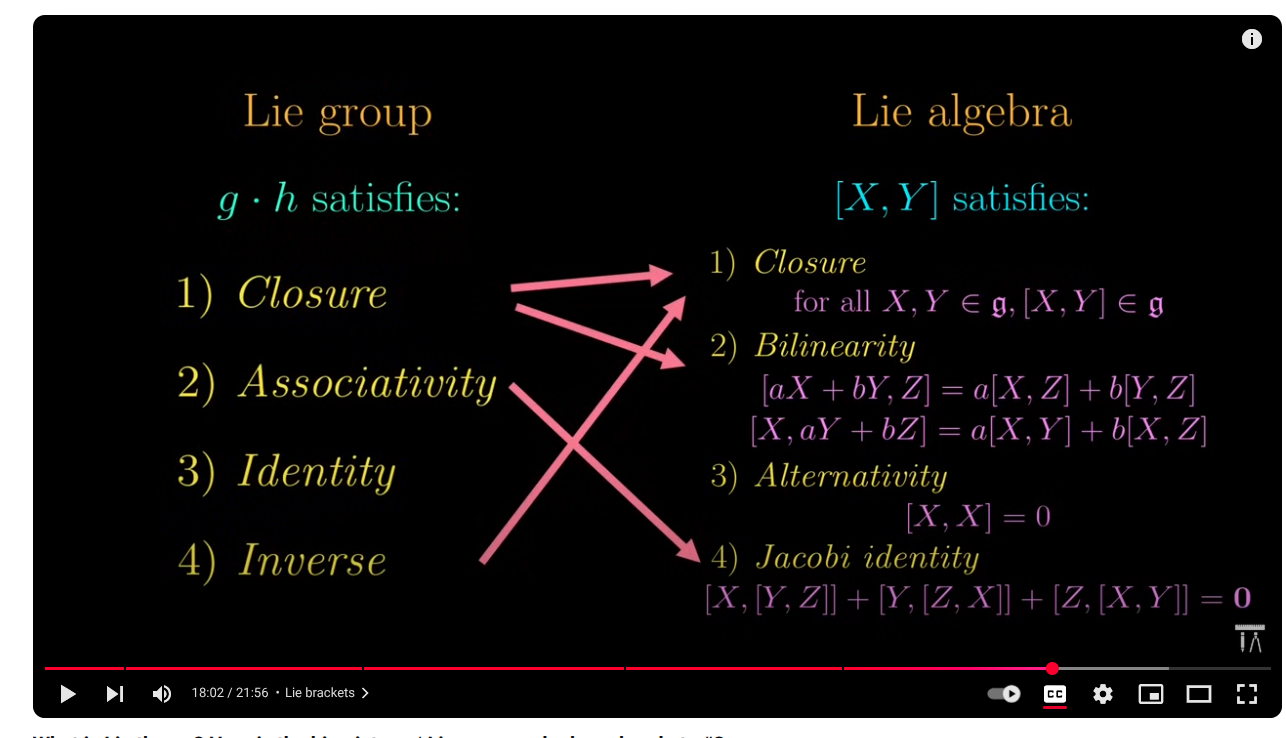
\includegraphics[scale=.4]{LieGroupVsLieBracket.png} 

\begin{remark}.

Many sources have pointed out that Lie Algebras are easier to manage/manipulate than Lie Groups, which makes them the focus of study.  One particular analogy was that the Lie Group is like a globe of the Earth while the Lie Algebra is the flat map that we use to represent it.

\end{remark}
\HLINE
\begin{remark}[\textbf{MathGTP}: What are the left-invariant vector spaces of $\R^2$?].

\begin{itemize}
\item Step 1: Understand the concept of left-invariant vector fields  
A left-invariant vector field on a Lie group \( G \) is a vector field \( X \) such that for every \( g, h \in G \), the following holds:  
\[ (L_g)_* X_h = X_{gh} \]  
where \( L_g \) is the left translation by \( g \) and \( (L_g)_* \) is its differential.  

\item Step 2: Identify the Lie group and its Lie algebra  
Here, \( G = \mathbb{R}^2 \), which is an abelian Lie group under addition. The Lie algebra \( \mathfrak{g} \) of \( \mathbb{R}^2 \) is also \( \mathbb{R}^2 \), with the trivial Lie bracket \([X, Y] = 0\) for all \( X, Y \in \mathfrak{g} \).  

\item Step 3: Determine the left-invariant vector fields  
For \( \mathbb{R}^2 \), left translation \( L_g \) is simply addition: \( L_g(h) = g + h \). The differential \( (L_g)_* \) is the identity map. Thus, a vector field \( X \) is left-invariant if:  
\[ X_{g + h} = X_h \]  
This implies \( X \) is constant, i.e., \( X = (a, b) \) for some \( a, b \in \mathbb{R} \). Therefore, the left-invariant vector fields on \( \mathbb{R}^2 \) are the constant vector fields.  

\item Step 4: Describe the space of left-invariant vector fields  
The space of left-invariant vector fields on \( \mathbb{R}^2 \) is isomorphic to \( \mathbb{R}^2 \) itself, spanned by the constant basis vector fields \( \partial_x \) and \( \partial_y \).
\item Final Answer
The left-invariant vector fields on \(\mathbb{R}^2\) are the constant vector fields, and the space of left-invariant vector fields is isomorphic to \(\mathbb{R}^2\).

\end{itemize}

\end{remark}

\HLINE
\begin{remark}[\textbf{MathGPT: }What are the left-invariant vector fields of $\GLG(n,\R)$?].

\begin{itemize}
\item \textbf{Step 1: Understanding GL(n,R) and Left-Invariant Vector Fields}
GL(n,R) is the general linear group of n x n invertible matrices with real entries, and it is a Lie group. A vector field \(X\) on a Lie group \(G\) is left-invariant if for every \(g \in G\), the pushforward of \(X\) by the left translation \(L_g\) is equal to \(X\). This means \((L_g)_* X = X\).

\item \textbf{Step 2: Identifying the Lie Algebra}
The space of left-invariant vector fields on a Lie group \(G\) is isomorphic to its Lie algebra \(\mathfrak{g}\), which is the tangent space at the identity element, \(T_e G\). For GL(n,R), the Lie algebra, denoted as \(\mathfrak{gl}(n,R)\), is the space of all n x n real matrices, \(M(n,R)\).

\item \textbf{Step 3: Associating Left-Invariant Vector Fields}
For any matrix \(A \in \mathfrak{gl}(n,R)\), we can associate a left-invariant vector field \(X_A\). For any \(g \in GL(n,R)\), the value of the vector field \(X_A\) at \(g\) is given by \(X_A(g) = (L_g)_* (A)\).

\item \textbf{Step 4: Calculating the Pushforward}
To understand \((L_g)_* (A)\), consider a curve \(\gamma(t)\) in GL(n,R) such that \(\gamma(0) = e\) and \(\gamma'(0) = A\). The pushforward \((L_g)_* (A)\) is the tangent vector to the curve \(L_g(\gamma(t)) = g\gamma(t)\) at \(t=0\). By computing the derivative, we find that the derivative at \(t=0\) is \(gA\).

\item \textbf{Step 5: Form of Left-Invariant Vector Fields}
Therefore, the left-invariant vector field \(X_A\) associated with \(A \in \mathfrak{gl}(n,R)\) is given by \(X_A(g) = gA\). The set of all left-invariant vector fields on GL(n,R) is \(\{X_A \mid A \in M(n,R)\}\), where \(X_A(g) = gA\).

\item \textbf{Step 6: Lie Algebra Structure}
These vector fields form a Lie algebra under the Lie bracket operation. If \(X_A\) and \(X_B\) are two left-invariant vector fields, then their Lie bracket \([X_A, X_B]\) is also a left-invariant vector field, corresponding to the matrix \([A, B] = AB - BA\). Thus, \([X_A, X_B] = X_{[A,B]}\).

\item \textbf{Final Answer}
The left-invariant vector fields of GL(n,R) are of the form \(X_A\), where \(A\) is an n x n real matrix, and \(X_A(g) = gA\) for any \(g \in GL(n,R)\). These vector fields span the Lie algebra of GL(n,R), which is the space of all n x n real matrices.
\end{itemize}
\end{remark}

\end{document}
